%& /Users/ziky/.cache/org-persist/30/b09e04-3955-44a5-8352-3c7632147cc5-c01017142739369138b3be1c13d58df0
% Created 2025-09-30 Tue 00:55
% Intended LaTeX compiler: pdflatex
\documentclass[11pt]{article}
\usepackage[utf8]{inputenc}
\usepackage[T1]{fontenc}
\usepackage{amsmath}
\usepackage{amssymb}
\usepackage{capt-of}
\usepackage{hyperref}
\setlength{\abovedisplayskip}{0pt}
\setlength{\belowdisplayskip}{0pt}
\usepackage[a4paper, margin=1in]{geometry}

%% ox-latex features:
%   !announce-start, !guess-pollyglossia, !guess-babel, !guess-inputenc,
%   maths, image, !announce-end.

\usepackage{amsmath}
\usepackage{amssymb}

\usepackage{graphicx}

%% end ox-latex features


% end precompiled preamble
\ifcsname endofdump\endcsname\endofdump\fi

\author{Ziky Zhang}
\date{\today}
\title{Worksheet \#5}
\hypersetup{
 pdfauthor={Ziky Zhang},
 pdftitle={Worksheet \#5},
 pdfkeywords={},
 pdfsubject={},
 pdfcreator={},
 pdflang={English}}
\begin{document}

\maketitle
\begin{enumerate}
\item Answer the following:
\begin{enumerate}
\item Calculate the potential difference \(V_b - V_a\) due to the infinite rod of uniform charge density λ, as shown below. Perform this calculation by directly integrating the electric field over a path between \(a\) and \(b\). \\
Two points \(a\) and \(b\), distances \(r_a\) and \(r_b\), respectively, away from a long rod
\begin{center}
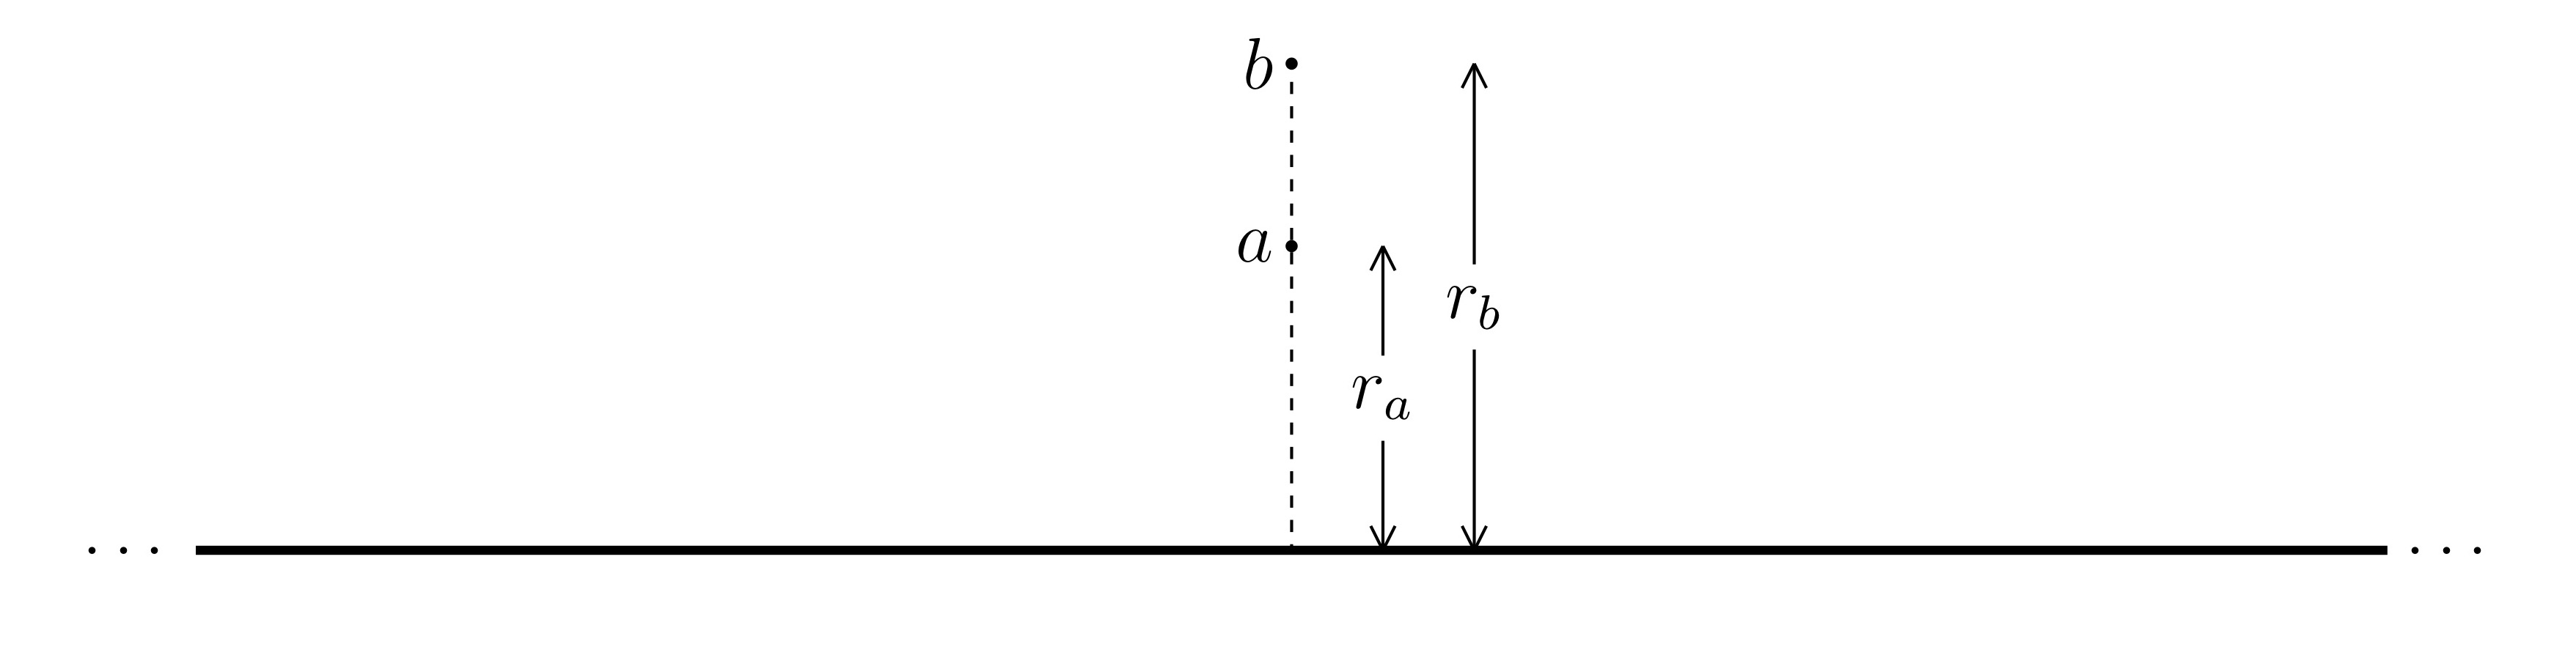
\includegraphics[height=3cm]{./img/5.1.jpg}
\end{center}
\item Calculate the potential difference \(V_b - V_a\) due to the rod of length \(L\) and uniform charge density \(\lambda\), as shown below. Perform this calculation by calculating \(Va\) and \(Vb\) directly from the charge distribution and subtracting. \\
Two points \(a\) and \(b\), distances \(r_a\) and \(r_b\), respectively from the center of a rod of length \(L\)
\begin{center}
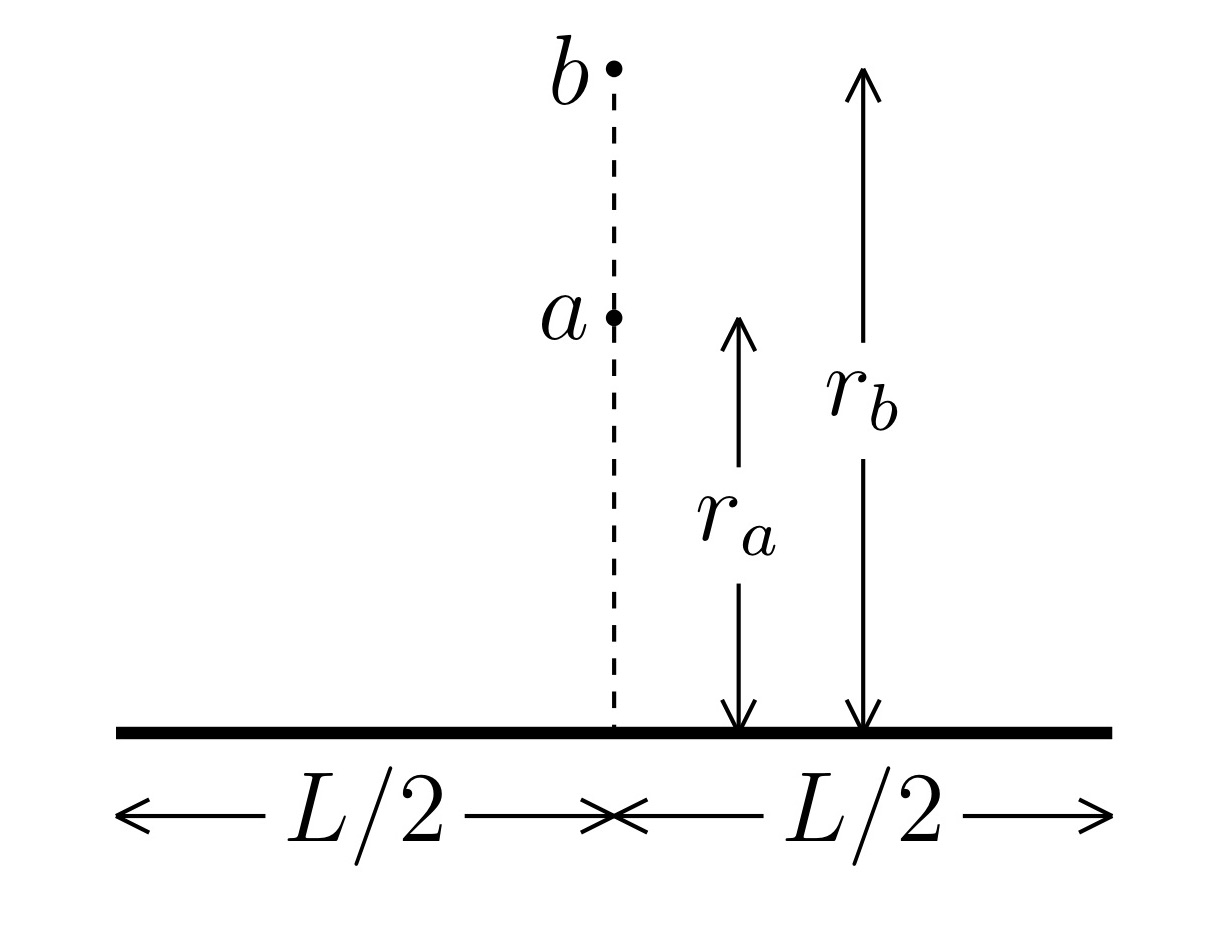
\includegraphics[height=3cm]{./img/5.2.jpg}
\end{center}
\item Show that your answer to part b matches your answer to part a in the \(\lim_{L\to\infty}\).
\end{enumerate}
\end{enumerate}

\newpage
1.(a)
\begin{align*}
V_b - V_a &= - \int_{r_a}^{r_b} E dr \\
          &= - \int_{r_a}^{r_b} \frac{\lambda}{2 \pi \epsilon_0 r} dr \\
          &= - \frac{\lambda}{2 \pi \epsilon_0} \int_{r_a}^{r_b} \frac{1}{r} dr \\
          &= - \frac{\lambda}{2 \pi \epsilon_0} \ln{r} \big|_{r_a}^{r_b} \\
          &= - \frac{\lambda}{2 \pi \epsilon_0} (\ln{r_b} - \ln{r_a}) \\
          &= - \frac{\lambda}{2 \pi \epsilon_0} \ln{\frac{r_{b}}{r_a}}
\end{align*}
\newline
1.(b)
\begin{align*}
\begin{aligned}[t]
V(r) &= \int_{0}^{L} E dr \\
     &= \int_{0}^{L} k_e \frac{\lambda dx}{\sqrt{r^2 + x^2}} \\
     &= k_e \lambda \int_{0}^{L} \frac{1}{\sqrt{r^2 + x^2}} dx \\
     &= k_e \lambda \ln \big(\big| \sqrt{x^2 + r^2} + x \big|\big)  \bigg|_{0}^{L} \\
     &= k_e \lambda \bigg( \ln \big( \sqrt{L^2 + r^2} + L \big) - \ln \big( \sqrt{0^2 + r^2} + 0 \big) \bigg) \\
     &= k_e \lambda \ln \bigg( \frac{ \sqrt{L^2 + r^2} + L }{r} \bigg)
\end{aligned}
\quad
\begin{aligned}[t]
V_b - V_a &= V(r) \big|_a^b \\
          &= k_e \lambda \ln \bigg( \frac{ \sqrt{L^2 + r_b^2} + L }{r_b} \cdot \frac{r_a}{ \sqrt{L^2 + r_a^2} + L }\bigg) \\
          &= k_e \lambda \ln \bigg( \frac{ \sqrt{L^2 + r_b^2} + L }{r_b} \cdot \frac{r_a}{ \sqrt{L^2 + r_a^2} + L }\bigg) \\
          &= k_e \lambda \ln \bigg( \frac{ r_a (\sqrt{L^2 + r_b^2} + L )}{r_b (\sqrt{L^2 + r_a^2} + L)} \bigg)
\end{aligned}
\end{align*}
\newline
\newline
1.(c) \\
\begin{align*}
\begin{aligned}[t]
\text{part b} \\
V_b - V_a &= \lim_{L \to \infty} V(r) \big|_a^b \\
          &= \lim_{L \to \infty} k_e \lambda \ln \bigg( \frac{ \sqrt{L^2 + r^2} + L }{r} \bigg) \bigg|_a^b\\
          &= k_e \lambda \ln \bigg( \frac{2L}{r} \bigg) \bigg|_a^b\\
          &= 2k_e \lambda \ln \bigg( \frac{L}{r} \bigg) \bigg|_a^b\\
          &= 2k_e \lambda \ln \bigg( \frac{L}{r_b} \cdot \frac{r_a}{L} \bigg) \\
          &= 2k_e \lambda \ln \frac{r_a}{r_b} \\
          &= \frac{\lambda}{2 \pi \epsilon_0} \ln \frac{r_a}{r_b} \\
\end{aligned}
\qquad
\begin{aligned}[t]
\text{part a} \\
V_b - V_a &= - \frac{\lambda}{2 \pi \epsilon_0} \ln{\frac{r_{b}}{r_a}} \\
          &= \frac{\lambda}{2 \pi \epsilon_0} \ln \frac{r_a}{r_b} \\
\\
\text{The an}& \text{swers for these two parts appears to agree}
\end{aligned}
\end{align*}
\end{document}
